\documentclass{article}
\usepackage{amsmath}
\usepackage{amssymb}
\usepackage{graphicx}
\usepackage{hyperref}
\usepackage[version=4]{mhchem}


\begin{document}
\section*{Problem}
In \(\triangle A B C\), angle \(C\) is a right angle. \(A C\) and \(B C\) are each equal to 1. \(D\) is the midpoint of \(A C . B D\) is drawn, and a line perpendicular to \(B D\) at \(P\) is drawn from \(C\). Find the distance from \(P\) to the intersection of the medians of \(\triangle A B C\).\\
\centering
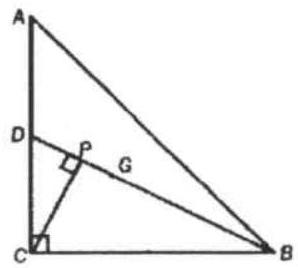
\includegraphics[width=\textwidth]{images/016(4).jpg}

\section*{Solution}
(D).\\
Method 1:\\
Let \(H\) be the foot of the perpendicular from \(E\) to \(D C\). Since \(C D=A B=5\), \(F G=2\), and \(\triangle F E G\) is similar to \(\triangle A E B\), we have\\
\(\frac{E H}{E H+3}=\frac{2}{5}\), so \(5 E H=2 E H+6\), and \(E H=2\). Hence Area \((\triangle A E B)=\frac{1}{2}(2+3) \cdot 5=\frac{25}{2}\).\\
\centering
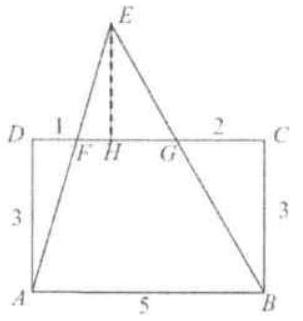
\includegraphics[width=\textwidth]{images/093.jpg}

Method 2:\\
Let \(I\) be the foot of the perpendicular from \(E\) to \(A B\). Since \(\triangle E I A\) is similar to \(\triangle A D F\) and \(\triangle E I B\) is similar to \(\triangle B C G\), we have \(A I / E I=1 / 3\) and \((5-A I) / E I=2 / 3\).\\
Adding gives \(5 / E I=1\), so \(E I=5\). The area of the triangle is \((1 / 2) \cdot 5 \cdot 5=25 / 2\).\\
\centering
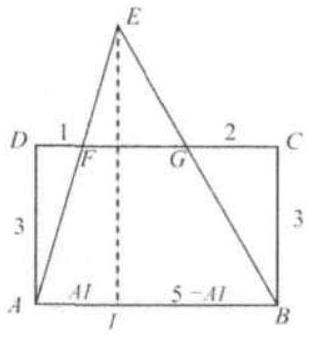
\includegraphics[width=\textwidth]{images/093(1).jpg}

\end{document}
